% Header
\renewcommand\evenpagerightmark{{\scshape\small Chapter 2}}
\renewcommand\oddpageleftmark{{\scshape\small Investigating the\si{TeV} scale}}

\renewcommand{\bibname}{References}

\hyphenation{}

\chapter[Investigating the\si{TeV} scale]%
{Investigating the\si{TeV} scale}
\label{chapt:2}

\section{The Standard Model of Particle Physics}
\label{chapt2:sec:SM}

\section{The \acl{LHC} \& the \acl{CMS}}
\label{chapt2:sec:LHC-CMS}

	Throughout its history, CERN has played a leading role in high energy particle physics. Large regional facilities such as CERN were thought after the second world war in an attempt to increase international scientific collaboration and allows scientists to share the forever increasing costs of experiment facilties required due to the need for increasing the energy in the center of mass to deeper probe matter. The construction of the first accelerators at the end of the 50s, the \acf{SC} and the \acf{PS}, was directly followed by the first observation of antinuclei in 1965~\cite{MASSAM1965}. Strong from the experience of the \acf{ISR}, the very first proton-proton collider that showed hints that protons are not elementary particles, the \acf{SPS} was built in the 70s to investigate the structure of protons, the preference for matter over antimatter, the state of matter in the early universe or exotic particles, and lead to the discovery in 1983 of the W and Z bosons~\cite{UA1W1983,UA2W1983,UA1Z1983,UA2Z1983}. These newly discovered particles and the electroweak intereaction would then be studied in details by the \acf{LEP} collider that will help to prove in 1989 that there only are three generations of elementary particles~\cite{ALEPH1989}. The LEP would then be dismantled in 2000 to allow for the LHC to be constructed in the existing tunnel.

	\subsection{LHC, the most powerful particle accelerator}
	\label{chapt2:ssec:LHC}
	
	The LHC has always been considered as an option to the future of CERN. At the moment of the construction of the LEP beneath the border between France and Switzerland, the tunnel was built in order to accomodate what would be a \acl{LHC} with a dipole field of \SI{10}{T} and a beam energy in between 8 and \SI{9}{TeV}~\cite{ANNUALREPORT1984} directly followed in 1985 with the creation of a 'Working Group on the Scientific and Technological Future of CERN' to investigate such a collider~\cite{ANNUALREPORT1985}. The decision was finally taken almost 10 years later, in 1994, to construct the LHC in the LEP tunnel~\cite{ANNUALREPORT1994} and the approval of the 4 main experiments that would take place at the 4 interaction points would come in 1997~\cite{ANNUALREPORT1997} and 1998~\cite{ANNUALREPORT1998}:
	
	\begin{itemize}
		\item[•] ALICE~\cite{ALICELOI} has been designed in the purpose of studying quark-gluon plasma that is believed to have been a state of matter that existed in the very first moment of the universe.
		\item[•] ATLAS~\cite{ATLASLOI} and CMS~\cite{CMSLOI} are general purpose experiements that have been designed with the goal of continuing the exploration of the Standard Model and investigate new physics.
		\item[•] LHCb~\cite{LHCBLOI} has been designed to investigate the preference of matter over antimatter in the universe through the CP violation.
	\end{itemize}
	
	These large scale experiments, as well as the full CERN accelerator complex, are displayed on Figure~\ref{fig:CERNComplex}.

	\begin{figure}[H]
		\centering
		\hspace*{-0.1\linewidth}
		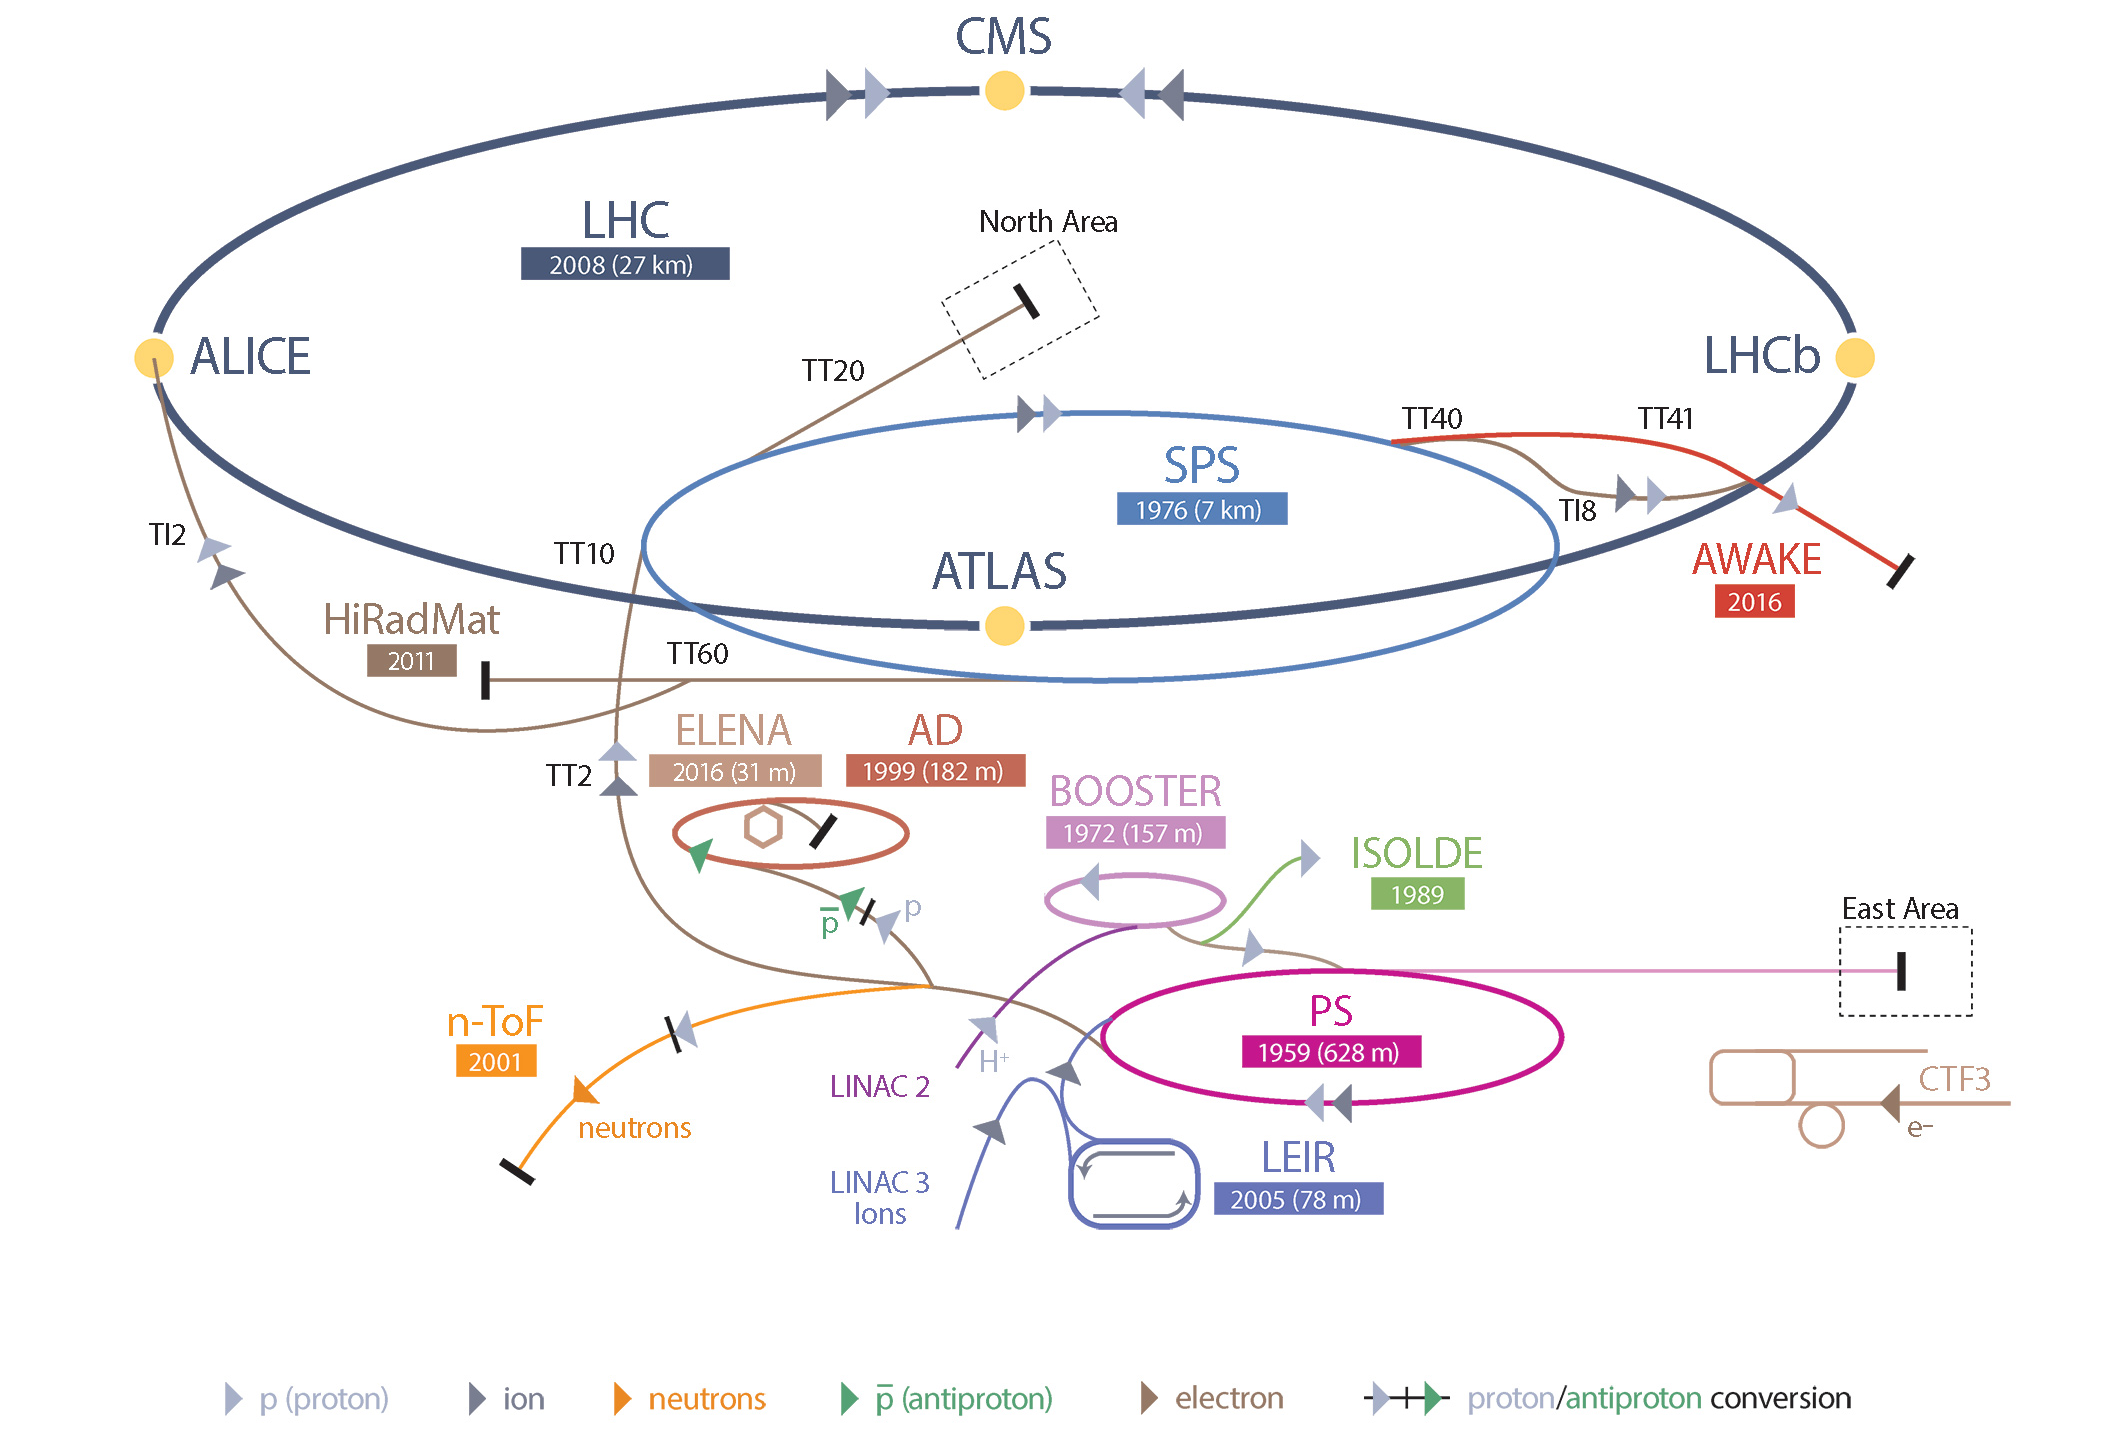
\includegraphics[width=1.2\linewidth]{fig/chapt2/CERN_Accelerator_Complex.png}
		\caption{\label{fig:CERNComplex} CERN accelerator complex.}
	\end{figure}
	
	The LHC is a \SI{27}{km} long hadron collider and the most powerful accelerator used for particle physics since 2008~\cite{LHC2008}.The LHC was originally designed to collide protons at a center-of-mass energy of \SI{14}{TeV} and luminosity of $10^{34}$ \si{cm^{-2}s^{-1}}, as well as $Pb$ ions at a center-of-mass energy of \SI{2.8}{TeV/A} with a peak luminosity of $10^{27}$ \si{cm^{-2}s^{-1}}. Run 1 of LHC was enough for both CMS and ATLAS to discover the Higgs boson~\cite{HIGGS2015} and for LHCb to discover pentaquarks~\cite{PENTAQUARK2015} and confirm the existance of tetraquarks~\cite{TETRAQUARK2017}. Nevertheless, after the \acf{LS3} (2024-2026), the accelerator will be in the so called \acf{HL-LHC} configuration~\cite{HLLHC2017}, increasing its instantaneous luminosity to $10^{35}$ \si{cm^{-2}s^{-1}} for $pp$ collisions and to $4.5\times 10^{27}$ \si{cm^{-2}s^{-1}}, boosting the discovery potential of the LHC.
	
		\subsubsection{Overview of LHC technology}
		\label{chapt2:sssec:LHCtechno}
	
	The two parrallel LHC beams are contained in a single twin-bore magnet because of the space restriction in the LEP tunnel that couldn't allow 2 completely separate proton rings to be built next to each other. The dipoles of the twin-bore magnets are showed in Figure~\ref{fig:LHCDipole} alongside the magnetic field generated along the dipole section to accelerate the particles. Quadrupoles, presented in Figure~\ref{fig:LHCQuadrupole}, are also used to focus to the beams.
	
	\begin{figure}[!h]
		\begin{subfigure}{\linewidth}
			\centering
			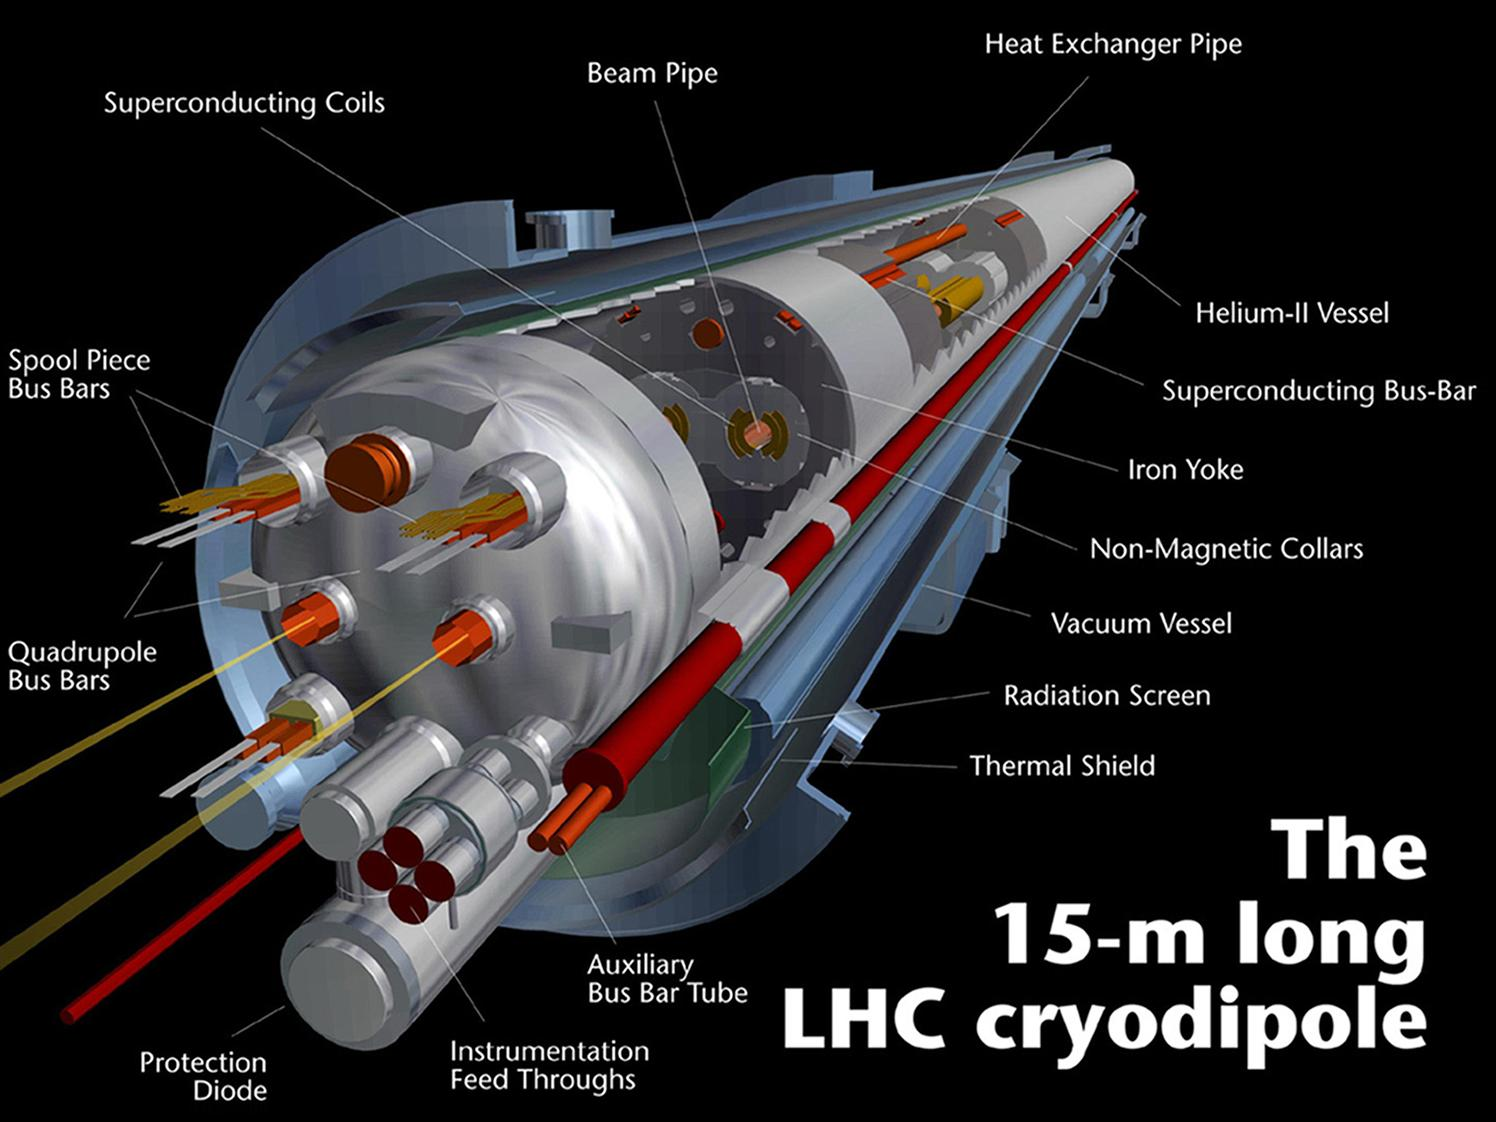
\includegraphics[width = 0.8\plotwidth]{fig/chapt2/LHC-dipole.jpg}\\
			\caption{\label{fig:LHCDipole:A}}
		\end{subfigure}
		\begin{subfigure}{\linewidth}
			\centering
			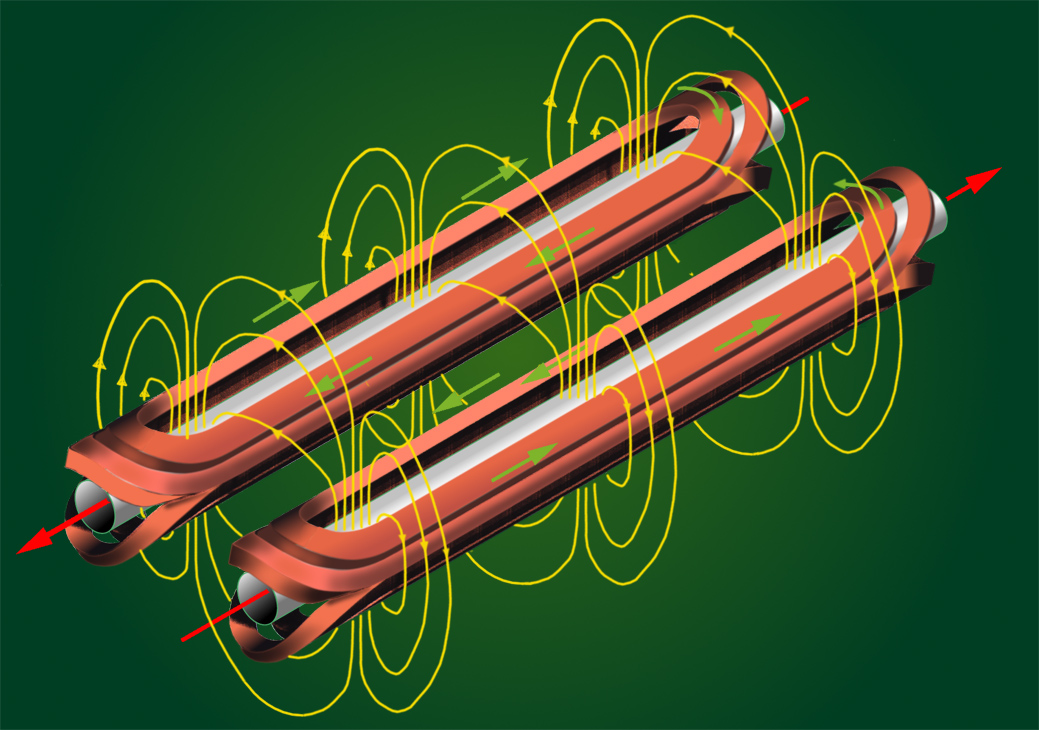
\includegraphics[width = 0.8\plotwidth]{fig/chapt2/LHC-dipole-field.jpg}
			\caption{\label{fig:LHCDipole:B}}
		\end{subfigure}
		\caption{\label{fig:LHCDipole} Figure~\ref{fig:LHCDipole:A}: schematics of the LHC cryodipoles. Figure~\ref{fig:LHCDipole:B}: magnetic field and resulting motion force applied on the beam particles.}
	\end{figure}
	
	\begin{figure}[!h]
		\begin{subfigure}{0.5\linewidth}
			\centering
			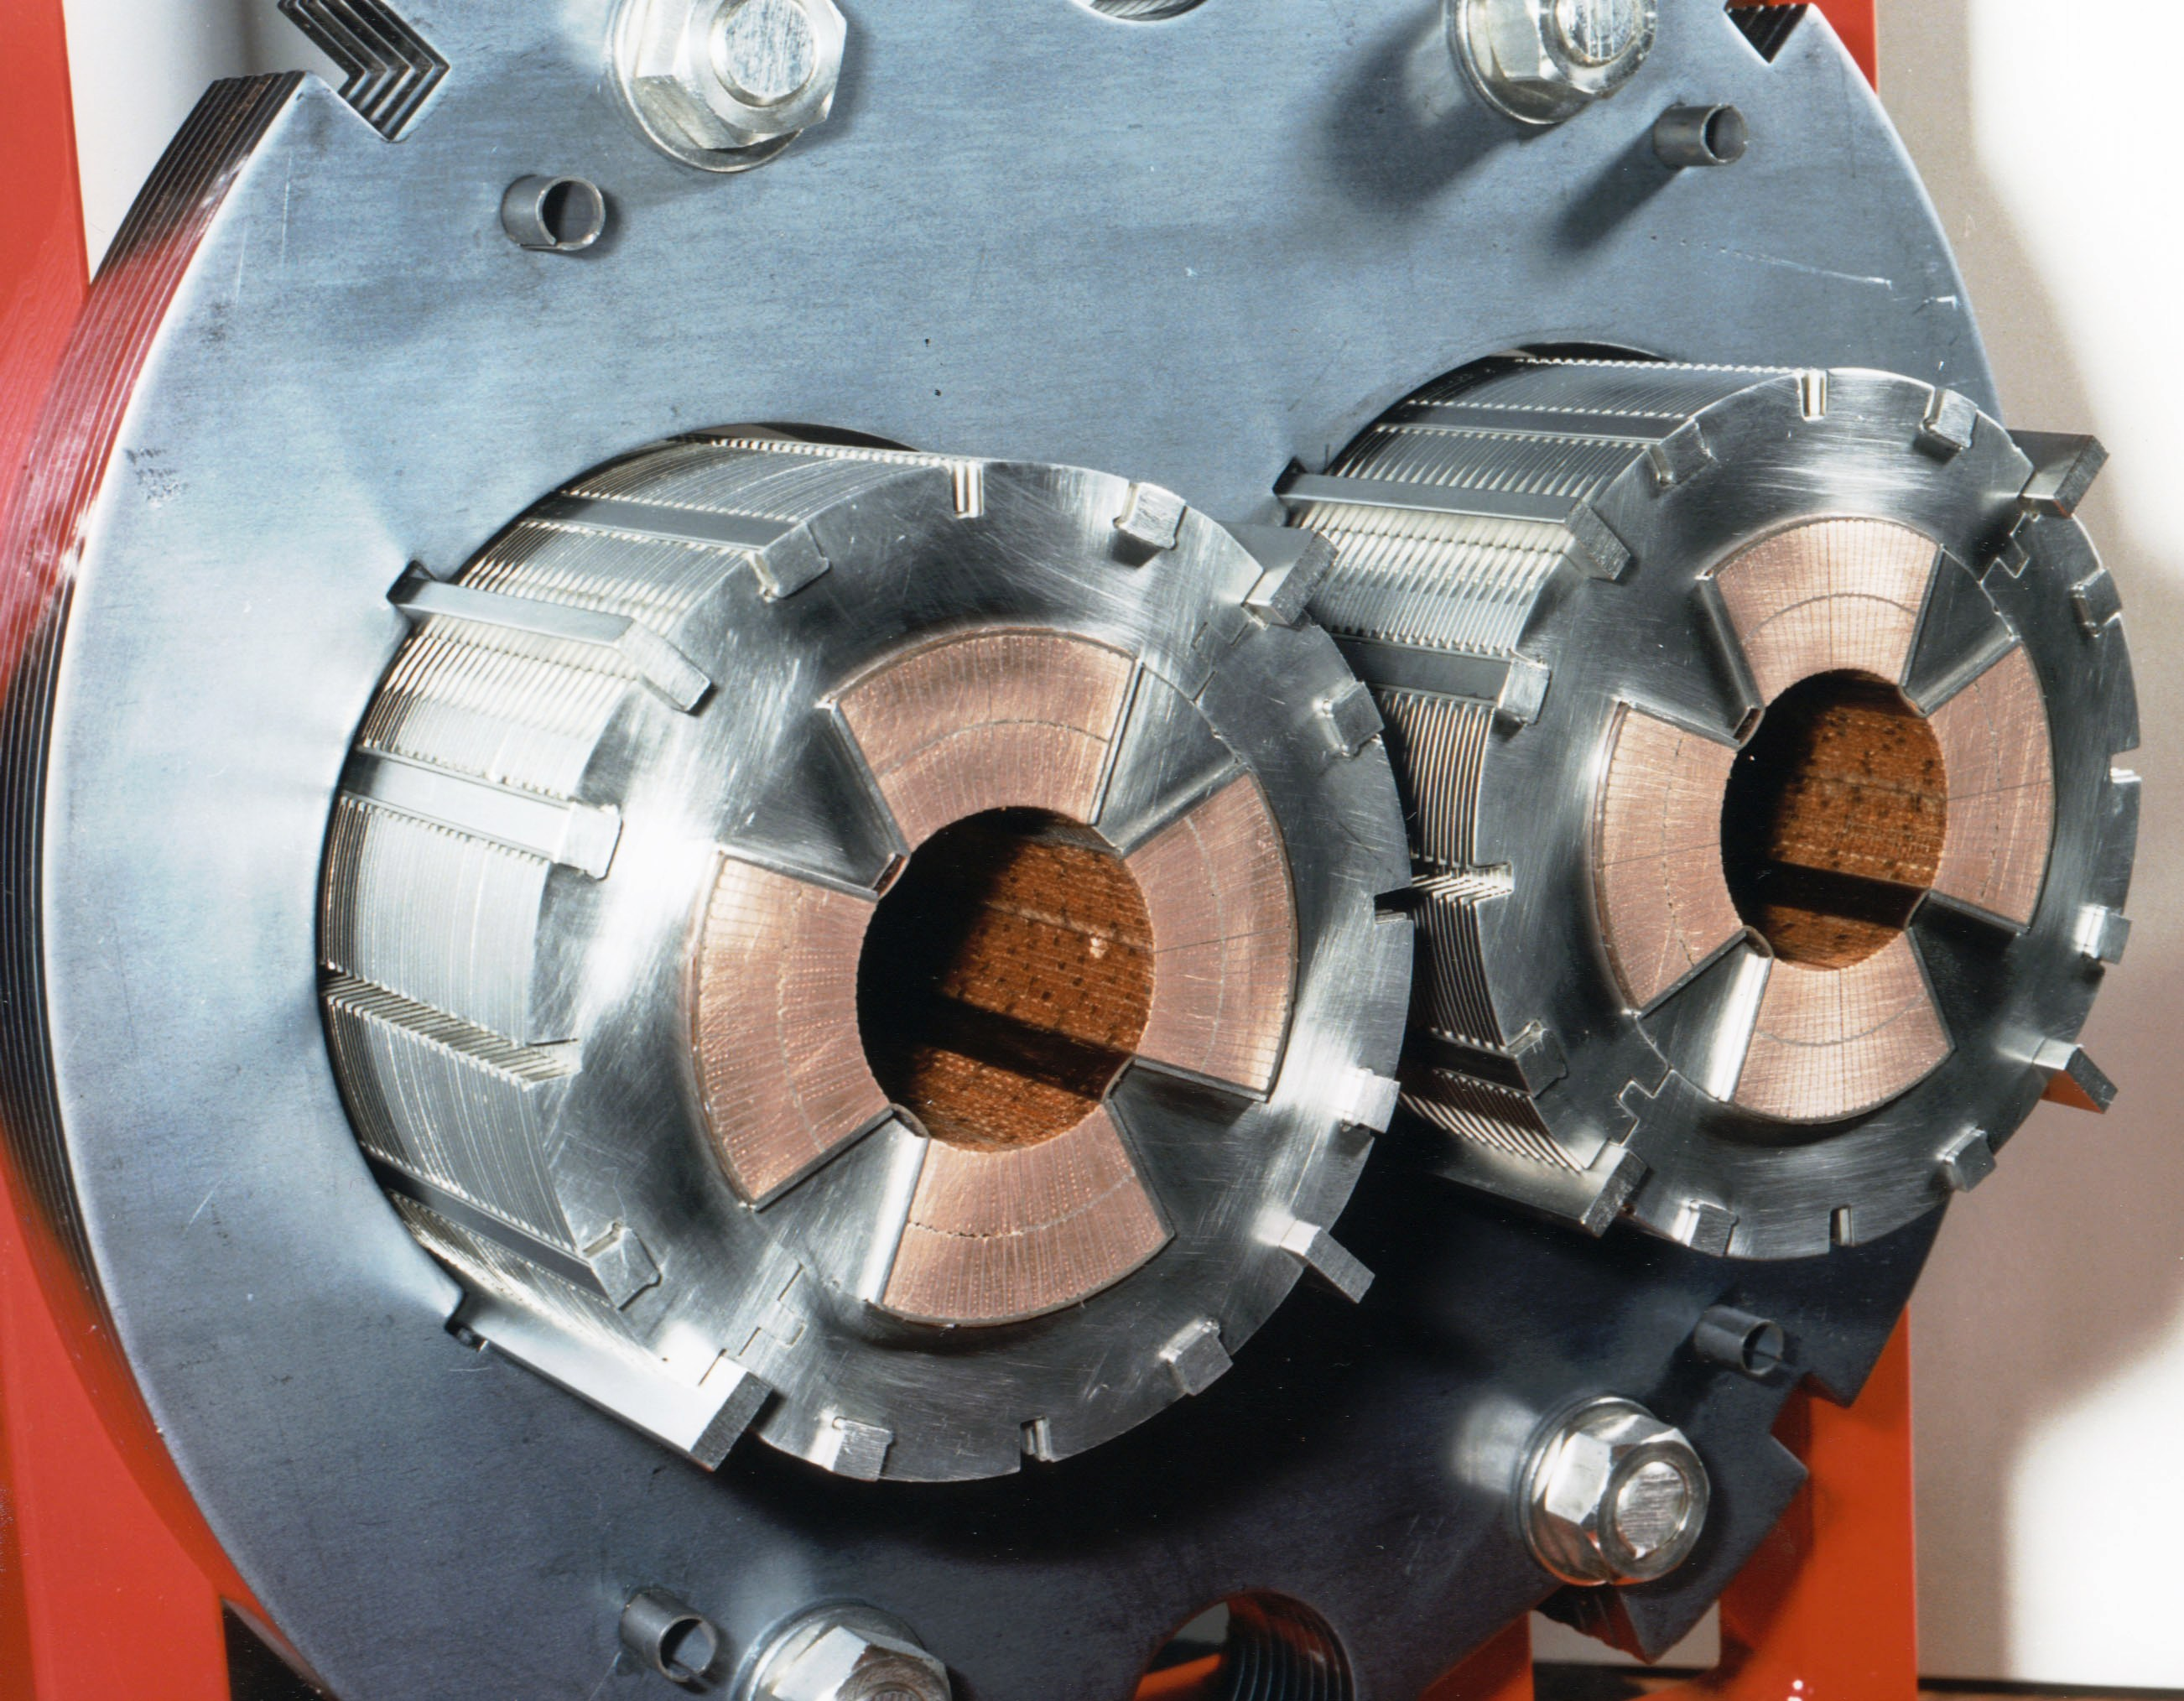
\includegraphics[width = 0.5\plotwidth]{fig/chapt2/LHC-quadrupole.jpg}
			\caption{\label{fig:LHCQuadrupole:A}}
		\end{subfigure}
		\begin{subfigure}{0.5\linewidth}
			\centering
			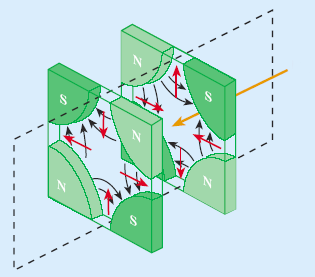
\includegraphics[width = 0.5\plotwidth]{fig/chapt2/LHC-quadrupole-field.png}
			\caption{\label{fig:LHCQuadrupole:B}}
		\end{subfigure}
		\caption{\label{fig:LHCQuadrupole} Figure~\ref{fig:LHCQuadrupole:A}: picture of the LHC quadrupoles. Figure~\ref{fig:LHCQuadrupole:B}: magnetic fields and resulting focussing force applied on the beam bunches by 2 consecutive quadrupoles.}
	\end{figure}

	\subsection{CMS, a multipurpose experiment}
	\label{chapt2:ssec:CMS}

\section{Muon Phase-II Upgrade}
\label{chapt2:sec:phase-2}

After the more than two years lasting \acf{LS1}, the \acf{LHC} delivered its very first Run-II proton-proton collisions early 2015. LS1 gave the opportunity to the LHC and to the its experiments to undergo upgrades. The accelerator is now providing collisions at center-of-mass energy of \SI{13}{TeV} and bunch crossing rate of \SI{40}{MHz}, with a peak luminosity exceeding its design value. During the first and upcoming second LHC Long Shutdown, the \acf{CMS} detector is also undergoing a number of upgrades to maintain a high system performance~\cite{MUONTDR}.

From the LHC Phase-2 or \acf{HL-LHC} period onwards, i.e. past the \acf{LS3}, the performance degradation due to integrated radiation as well as the average number of inelastic collisions per bunch crossing, or pileup, will rise substantially and become a major challenge for the LHC experiments, like CMS that are forced to address an upgrade program for Phase-II~\cite{PHASEIITP}. Simulations of the expected distribution of absorbed dose in the CMS detector under HL-LHC conditions, show in figure~\ref{fig:Dose} that detectors placed close to the beamline will have to withstand high irradiation, the radiation dose being of the order of a few tens of\si{Gy}.

\begin{figure}[H]
	\centering
	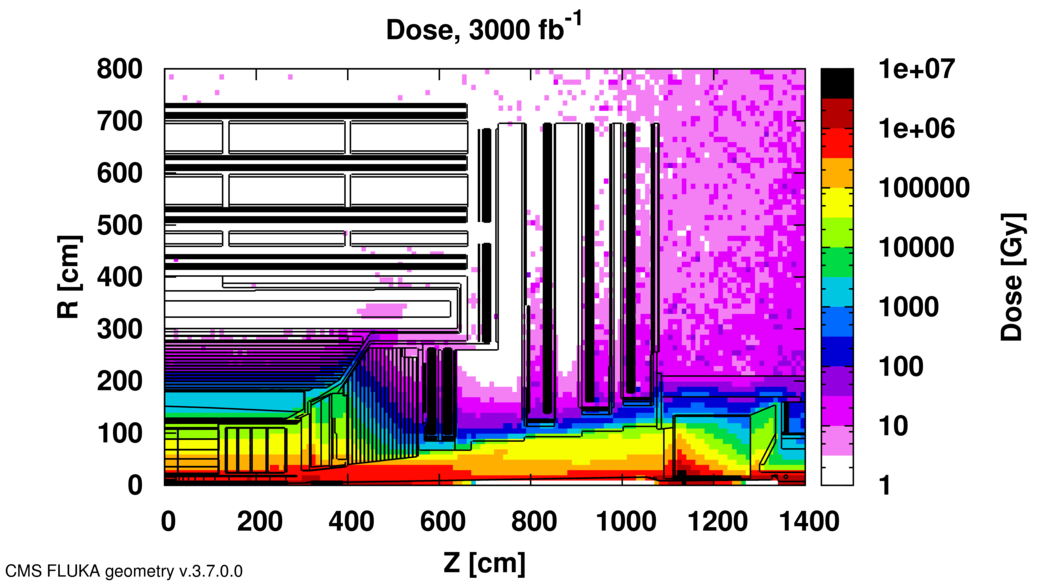
\includegraphics[width=0.7\textwidth]{fig/chapt2/HL-LHC-Dose.png}
	\caption{\label{fig:Dose} Absorbed dose in the CMS cavern after an integrated luminosity of \SI{3000}{\femto\per\barn}. R is the transverse distance from the beamline and Z is the distance along the beamline from the Interaction Point at Z=0.}
\end{figure}

The measurement of small production cross-section and/or decay branching ratio processes, such as the Higgs boson coupling to charge leptons or the $B_s \longrightarrow \mu^+\mu^-$ decay, is of major interest and specific upgrades in the forward regions of the detector will be required to maximize the physics acceptance on the largest possible solid angle. To ensure proper trigger performance within the present coverage, the muon system will be completed with new chambers. In figure~\ref{fig:Quadrant} one can see that the existing \acfp{CSC} will be completed by \acfp{GEM} and \acfp{RPC} in the pseudo-rapidity region $1.6<\vert\eta\vert<2.4$ to complete its redundancy as originally scheduled in the CMS Technical Proposal~\cite{CMSTP}.

\begin{figure}[H]
	\centering
	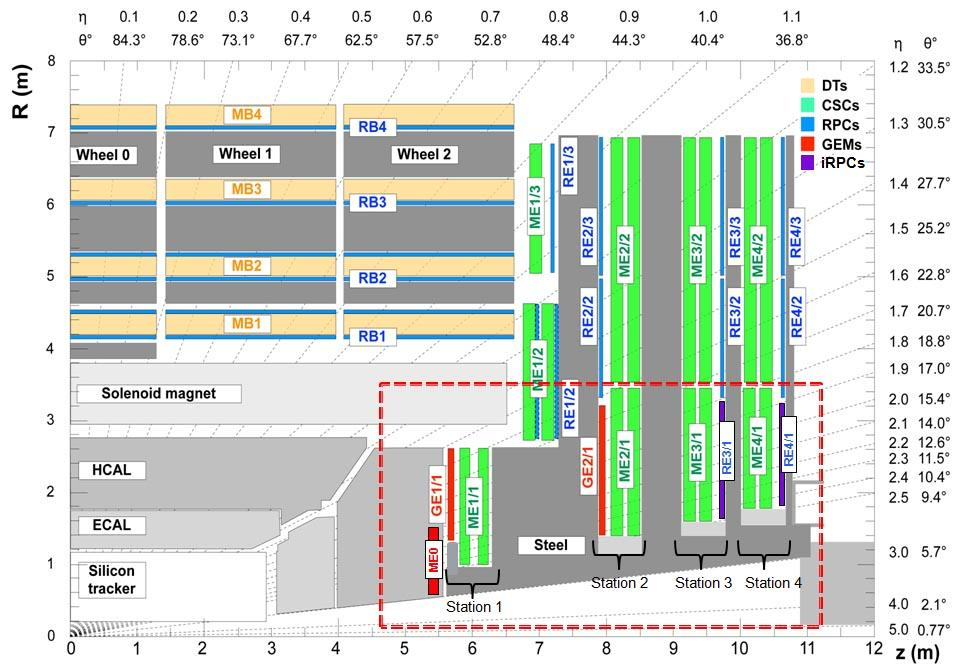
\includegraphics[width=0.7\textwidth]{fig/chapt2/MuonUpgrade-Plans.jpg}
	\caption{\label{fig:Quadrant} A quadrant of the muon system, showing DTs (yellow), RPCs (light blue), and CSCs (green). The locations of new forward muon detectors for Phase-II are contained within the dashed box and indicated in red for GEM stations (ME0, GE1/1, and GE2/1) and dark blue for improved RPC (iRPC) stations (RE3/1 and RE4/1).}
\end{figure}

RPCs are used by the CMS first level trigger for their good timing performances. Indeed, a very good bunch crossing identification can be obtained with the present CMS RPC system, given their fast response of the order of \SI{1}{ns}. In order to contribute to the precision of muon momentum measurements, muon chambers should have a spatial resolution less or comparable to the contribution of multiple scattering~\cite{MUONTDR}. Most of the plausible physics is covered only considering muons with $p_T<$\SI{100}{GeV} thus, in order to match CMS requirements, a spatial resolution of $\mathcal{O}$(few $\mathrm{mm}$) the proposed new RPC stations, as shown by the simulation in figure~\ref{fig:MultiScat}. According to preliminary designs, RE3/1 and RE4/1 readout pitch will be comprised between 3 and \SI{6}{mm} and 5 $\eta$-partitions could be considered.

\begin{figure}[H]
	\centering
	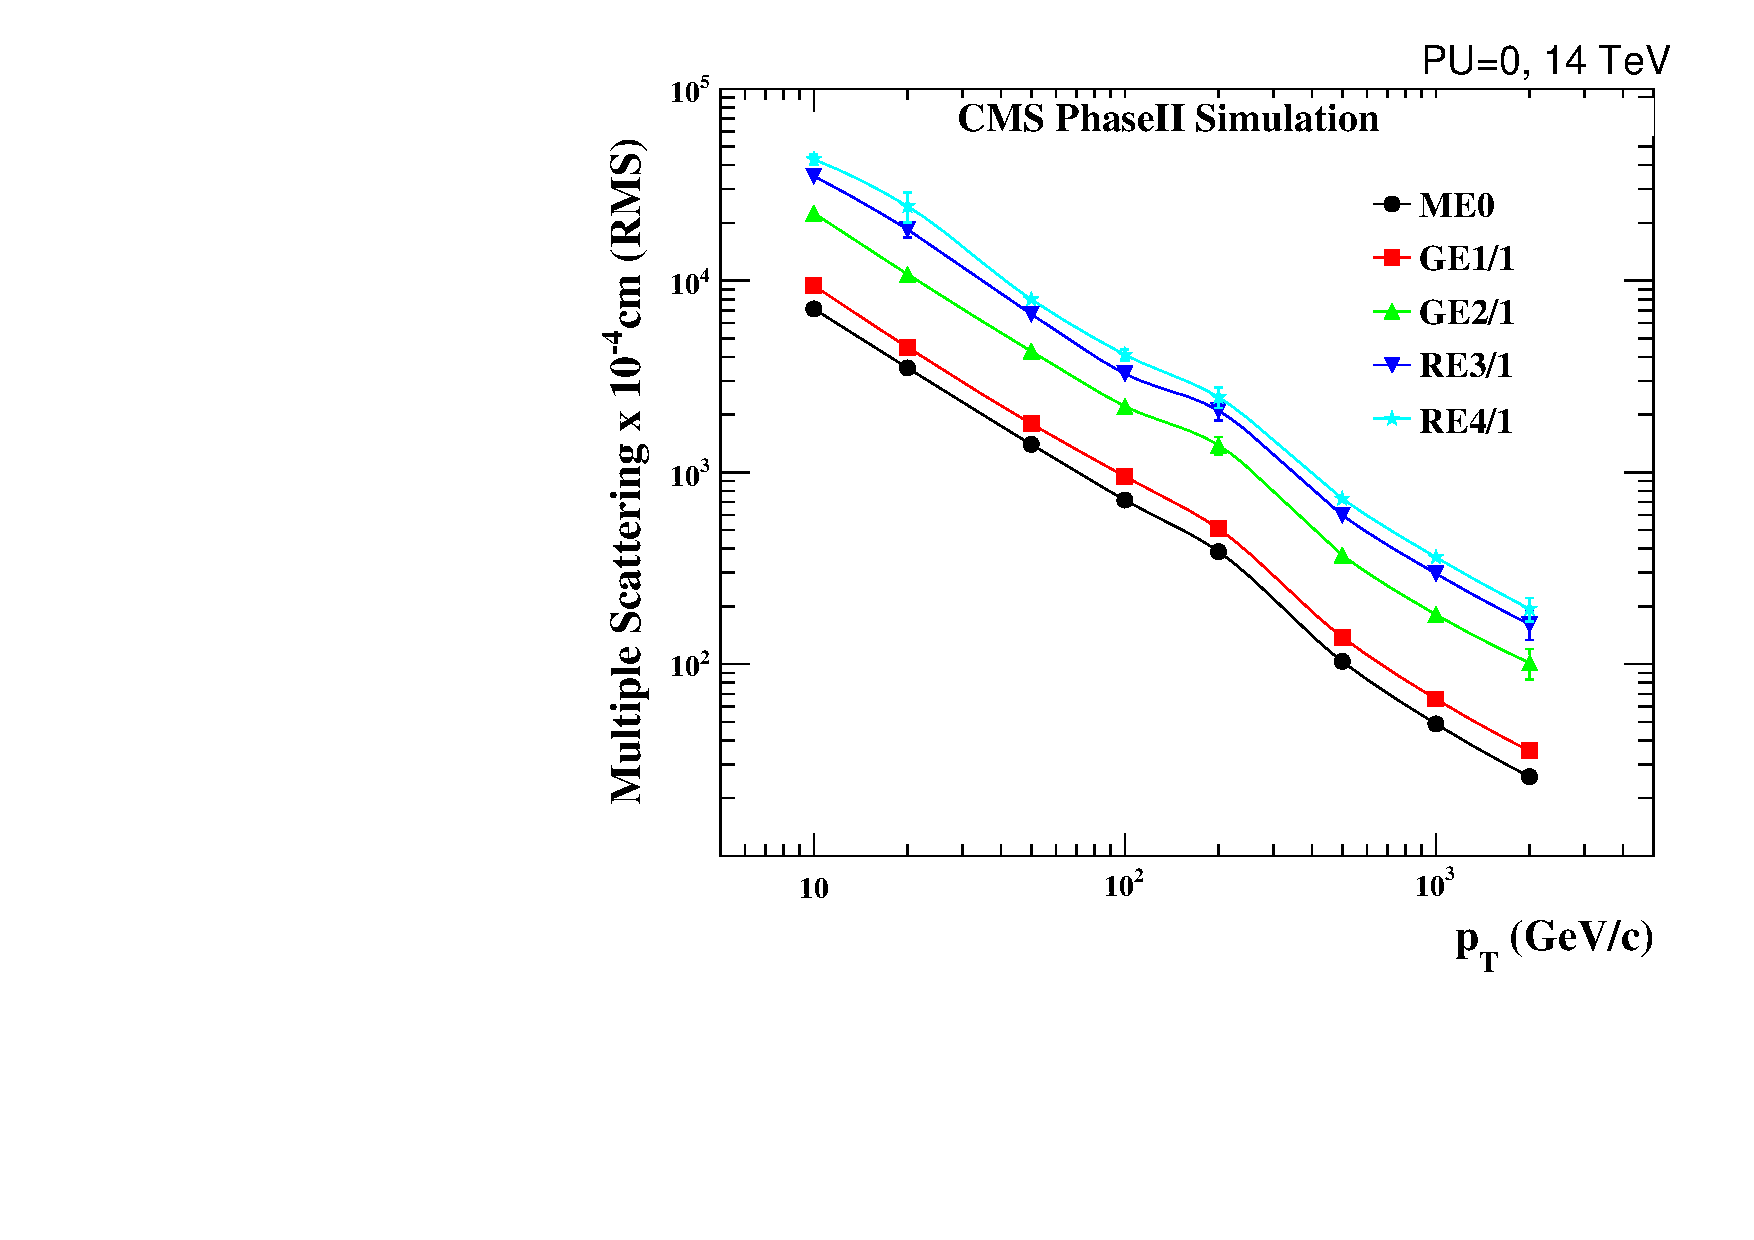
\includegraphics[width=0.6\textwidth]{fig/chapt2/MS_allstations.pdf}
	\caption{\label{fig:MultiScat}  RMS of the multiple scattering displacement as a function of muon $p_T$ for the  proposed forward muon stations. All of the electromagnetic processes such as bremsstrahlung and magnetic field effect are included in the simulation.}
\end{figure}

\clearpage{\pagestyle{empty}\cleardoublepage}
